\documentclass{article}

%% Denote paragraphs with vertical space rather than indenting (not critical)
\usepackage{parskip}

%% Support for URL in introductory text (not needed for main example)
\usepackage{url}

%% *** Enable PGFPLOTS (automatically enables TikZ) ***
\usepackage{pgfplots}

%% Prevent some PGFPLOTS messages (not critical)
\pgfplotsset{compat=1.18,compat/show suggested version=false}


\begin{document}

%% Introductory Text
Example 10.13 from the book\\
\emph{Unlocking LaTeX Graphics: A Concise Guide to Ti$k$Z/PGF and PGFPLOTS}.\\
For more information, visit \url{https://latex-graphics.com}.
\par\bigskip

%% *** START OF EXAMPLE CODE ***
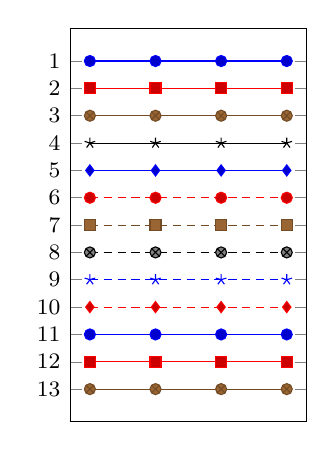
\begin{tikzpicture}
  \begin{axis}[
      scale only axis, width=3cm, height=5cm,
      font=\footnotesize, y dir=reverse,
      xtick=\empty, ytick={1,2,...,13},
      every axis plot/.style={samples=4},
      cycle list name=color, % PGFPLOTS default
    ]
    \foreach \n in {1,2,...,13} {
      \addplot expression {\n};
    }
  \end{axis}
\end{tikzpicture}
%% *** END OF EXAMPLE CODE ***

\end{document}
